\definecolor{mycolor1}{rgb}{0.00000,0.44700,0.74100}%
%
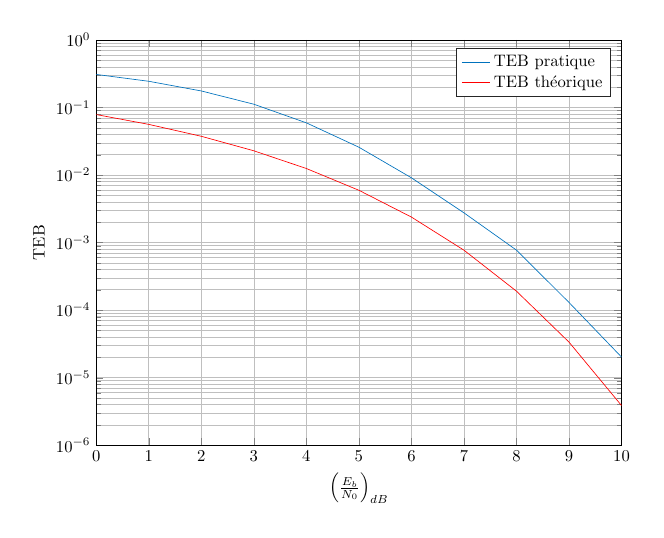
\begin{tikzpicture}[scale=0.60]

\begin{axis}[%
width=5in,
height=4in,
at={(1.011111in,0.641667in)},
xmin=0,
xmax=10,
xlabel={$\left(\frac{E_b}{N_0}\right)_\text{dB}$},
xmajorgrids,
ymode=log,
ymin=1e-06,
ymax=1,
yminorticks=true,
ylabel={TEB},
ymajorgrids,
yminorgrids,
legend style={legend cell align=left,align=left,draw=white!15!black}
]
\addplot [color=mycolor1,solid]
  table[row sep=crcr]{%
0	0.30887875\\
1	0.244597857142857\\
2	0.175844642857143\\
3	0.111914464285714\\
4	0.0593260714285714\\
5	0.0258430357142857\\
6	0.00910785714285714\\
7	0.002759285714286\\
8	0.000774107142857143\\
9	0.00013\\
10	2.0195640679161e-05\\
};
\addlegendentry{TEB pratique};

\addplot [color=red,solid]
  table[row sep=crcr]{%
0	0.0786496035251426\\
1	0.0562819519765415\\
2	0.037506128358926\\
3	0.0228784075610853\\
4	0.0125008180407376\\
5	0.00595386714777866\\
6	0.00238829078093281\\
7	0.000772674815378444\\
8	0.000190907774075993\\
9	3.36272284196175e-05\\
10	3.87210821552204e-06\\
};
\addlegendentry{TEB théorique};

\end{axis}
\end{tikzpicture}%